\section{Data driven model and prediction}

This section will present a method for heat demand prediction base on machine learning technique.

%\subsection{Parameters estimation.}

\subsection{LSTM model.}

Long short term memory model or LSTM is a very special kind of recurrent neural network which used in application such as speech recognition, language modeling, translation, text generation ..etc. Christopher Olah gave an excellent explanation on LSTM model and how does it work in her blog. \cite{LSTM}.The structure of LSTM model can be seen in figure \ref{fig:LSTM}.

There are many types of LSTM models that can be used for each specific type of time series forecasting problem.These are problems comprised of series of observations and a model is required to learn from the series of past observations to predict the next value in the sequence.

\begin{figure}[H]
	\centering
	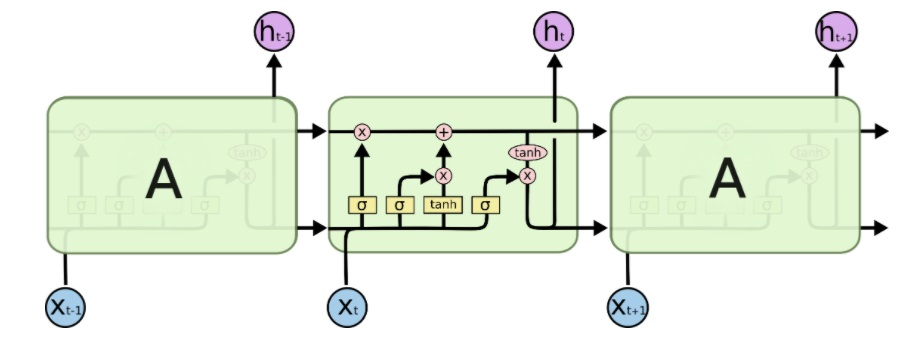
\includegraphics[width=1.0\columnwidth]{Pictures/LSTM strcuture.jpg}
	\caption[Short title]{LSTM model strcuture}
	\label{fig:LSTM}
	\end{figure}


In this study an multivariate LSTM model has been developed using Pytorch (Facebook famous machine learning open source library) for heat demand prediction inside a dwelling. The goal of this study is showing a proof of concept on how the model can learn the dynamic behaviour of different house.

The data has been generated from house simulation model and NEN-2018 weather data file. The first 70\% is used for training and  30\% left for validation.

\subsection{Model Prediction}

The model can predict the next hours heat demand base on the previous 12 hours pass inputs data. The inputs data consist of: 

\begin{itemize}
    \item $T_{a}$: Ambient temperature $[^o C]$.
    \item $SP$   : The temperature set point profile$[^o C]$. 
    \item $\dot{Q}_{Solar}$: Heat generated from solar irradiation $[W/m^2]$.
    \item $\dot{Q}_{inernal}$: Internal heat gain from the present people and furniture inside the house [W].
    \item $\dot{Q}_{inst}$: delivered heat from heating system (radiator) [W].
\end{itemize}

The simulation result in figure \ref{fig:heat demand prediction} and \ref{fig:50 days heat demand prediction} show that the model give a good prediction for an hour figure \ref{fig:heat demand prediction} and multiple hours figure \ref{fig:50 days heat demand prediction} heat demand.

\begin{figure}[H]
	\centering
	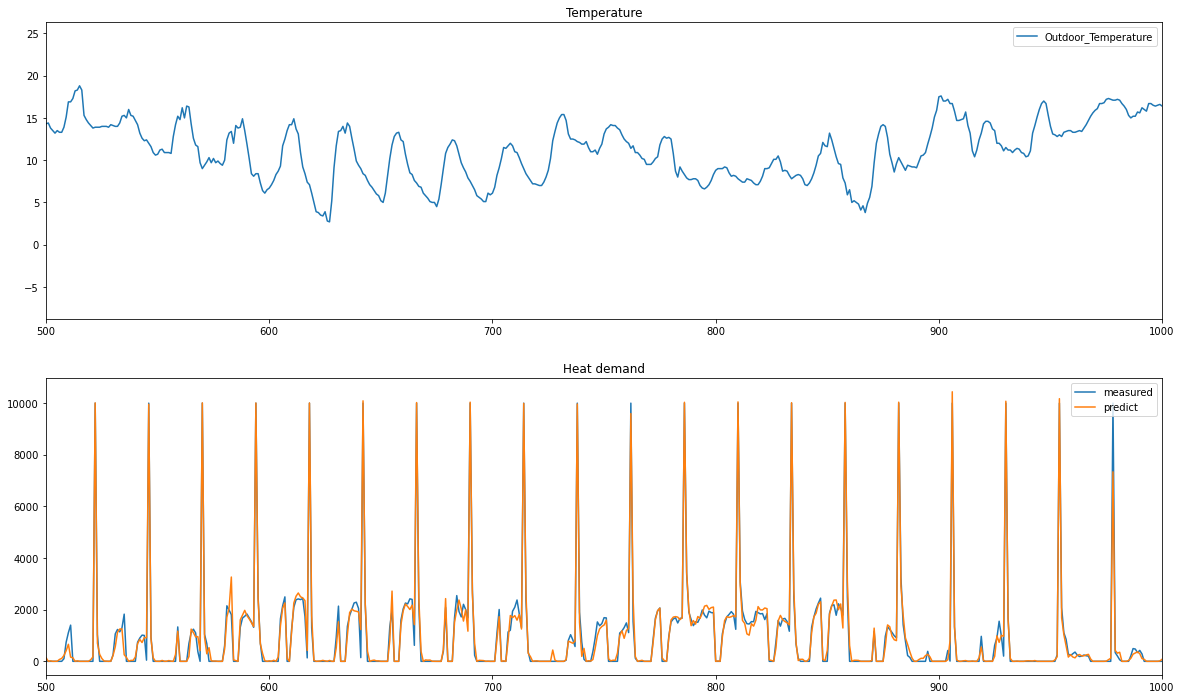
\includegraphics[width=1.0\columnwidth]{Pictures/house heat demand prediction zoom.png}
	\caption[Short title]{Heat demand prediction for light weight construction.}
	\label{fig:heat demand prediction}
	\end{figure}

The simulation result in figure \ref{fig:heat demand prediction} shows that the model give a good prediction for the next hour heat demand needed.

\begin{figure}[H]
	\centering
	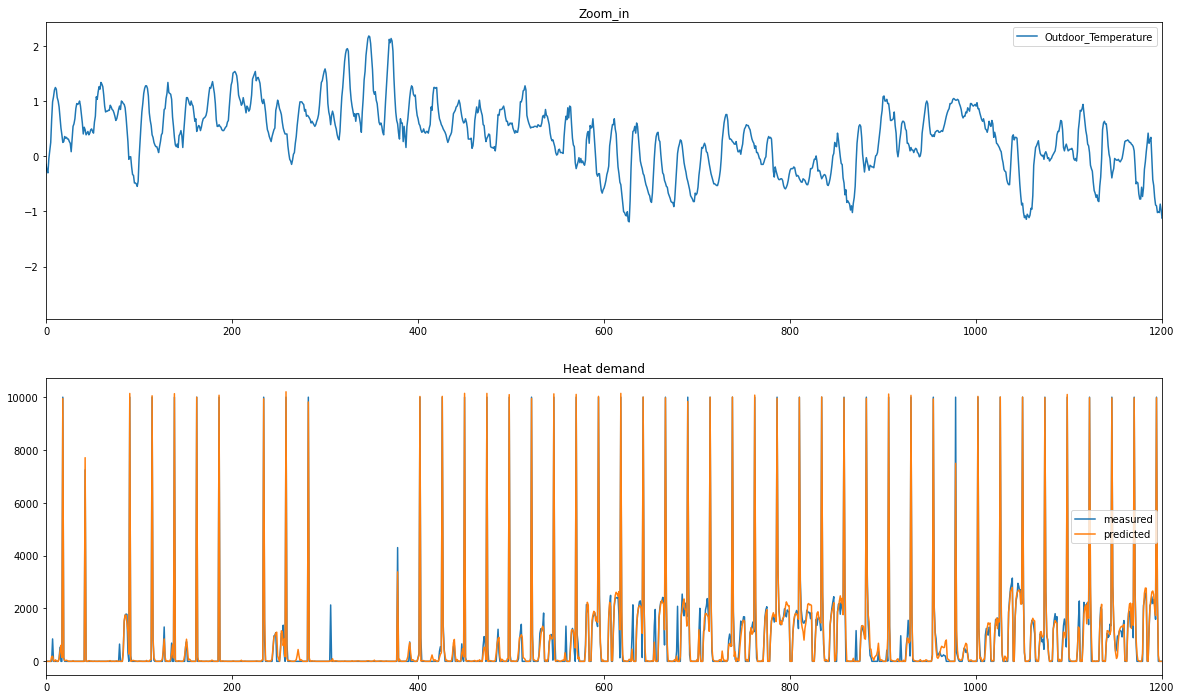
\includegraphics[width=1.0\columnwidth]{Pictures/50days_heat_demand_prediction.png}
	\caption[Short title]{50 days heat demand prediction.}
	\label{fig:50 days heat demand prediction}
	\end{figure}


The prediction above has based on the assumption that all the parameters such as $T_{a}$, $SP$, $\dot{Q}_{Solar}$, $\dot{Q}_{inernal}$ and $\dot{Q}_{inst}$ for the pass and current time are well known. The result show that the prediction accuracy reduce if solar power and internal heat gain at the current time are not known (in this simulation solar power and internal heat gain are set to zero) figure \ref{fig:hour prediction with uncertainties}.

\begin{figure}[H]
	\centering
	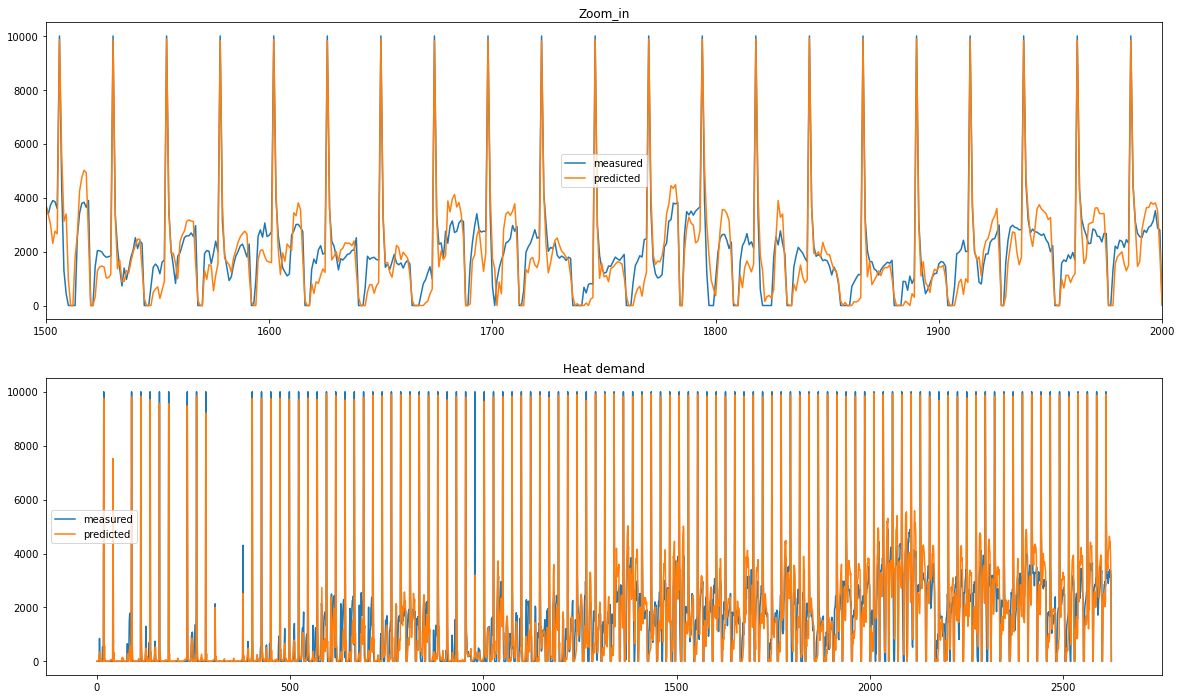
\includegraphics[width=1.0\columnwidth]{Pictures/1hour_heatdemand_with_uncertainties.png}
	\caption[Short title]{1 hour heat demand prediction with uncertainties}
	\label{fig:hour prediction with uncertainties}
	\end{figure}
	
In summary, to be able to have a good heat demand prediction, the model need to be trained with a good data sources which can represent the dynamic behaviour of the house in all scenarios. The more data in different situations use for the training step the more accurate the prediction is.   

\newpage